\documentclass[11pt]{beamer}
% Soporte para los acentos.
\usepackage[utf8]{inputenc}
\usepackage[T1]{fontenc}    
% Idioma español.
\usepackage[spanish,mexico, es-tabla]{babel}
\usepackage{amsmath}
\usepackage{amsfonts}
\usepackage{amssymb}
\usepackage[caption=false]{subfig}
\usepackage{graphicx}
\usepackage{lipsum}
\usepackage{ragged2e}
\usepackage{hyperref}
\usepackage{url}
\usepackage{listings}
\usepackage{xcolor}

\definecolor{codegreen}{rgb}{0,0.6,0}
\definecolor{codegray}{rgb}{0.5,0.5,0.5}
\definecolor{codepurple}{rgb}{0.58,0,0.82}
\definecolor{backcolour}{rgb}{0.95,0.95,0.92}

\lstdefinestyle{mystyle}{
    backgroundcolor=\color{backcolour},   
    commentstyle=\color{codegreen},
    keywordstyle=\color{magenta},
    numberstyle=\tiny\color{codegray},
    stringstyle=\color{codepurple},
    basicstyle=\ttfamily\footnotesize,
    breakatwhitespace=false,         
    breaklines=true,                 
    captionpos=b,                    
    keepspaces=true,                 
    numbers=left,                    
    numbersep=5pt,                  
    showspaces=false,                
    showstringspaces=false,
    showtabs=false,                  
    tabsize=2
}

\lstset{style=mystyle}

\usetheme{Madrid}
\newcommand{\celda}[1]{
	\begin{minipage}{3cm}
		\vspace{5mm}
		#1
		\vspace{5mm}
	\end{minipage}
}

\author{Tania Michelle Rubí Rojas}
\title[Music Genre Classification]{GTZAN Dataset - Music Genre Classification}
\date{\today} 
\subtitle{Proyecto Final}
\institute[UNAM]{Facultad de Ciencias, UNAM}

\begin{document}
\begin{frame}
    \maketitle
\end{frame}

\begin{frame}{Contenido}
    \tableofcontents
\end{frame}

\section{Objetivo}
\begin{frame}{Objetivo}
    \justifying
    \textbf{Dada una canción, queremos saber a qué genero musical pertenece.}
    
    Para atacar este problema, utilizaremos dos \textit{modelos} de 
    clasificación diferentes:
    \begin{enumerate}
        \item SVC (Support-Vector Clustering)
        
        Se explicará el preprocesamiento de los datos antes de usar SVC, y su 
        precisión al momento de clasificar canciones.
        
        \item PCA/SVC (Principal Component Analysis/ Singular Vector Clustering)
        
        Se explicará el preprocesamiento necesario para poder aplicar PCA y la
        precisión de este nuevo modelo al momento de clasificar canciones.
    \end{enumerate}
\end{frame}
	
\section{Materiales}
\begin{frame}{Conjunto de Datos}
    \justifying
    El conjunto de canciones que utlizaremos para entrenar nuestros modelos
    se obtuvo del sitio web \textit{Kaggle}
    \begin{center}
        \url{https://www.kaggle.com/andradaolteanu/gtzan-dataset-music-genre-classification}
    \end{center}
\end{frame}

\begin{frame}{Conjunto de Datos}
    \justifying
    el cual contiene $2$ archivos y $2$ carpetas (pero sólo nos enfocaremos en el 
    primer archivo):
    \begin{enumerate}
        \item \textit{features\_30\_sec.csv}

        Contiene un conjunto de datos con $60$ atributos (características
        basadas en el timbre):
        \begin{itemize}
            \item \textbf{filename}: el nombre del archivo.
            \item \textbf{length}:  el tamaño del archivo.
            \item \textbf{spectral\_bandwidth}: el ancho de banda espectral.
            \item \textbf{spectral\_centroid}: el centroide espectral.
            \item \textbf{rms}: el nivel promedio de una onda (en el espectro).
            \item \textbf{label}: el género musical al cual pertenece.
        \end{itemize}

        con $1000$ entradas ($10$ por cada género)
    \end{enumerate}
\end{frame}

\begin{frame}{Conjunto de Datos}
    Tenemos $10$ géneros musicales: blues, clásica, country, disco, hiphop, 
    jazz, metal, pop, reggae, rock.
    \begin{center}
        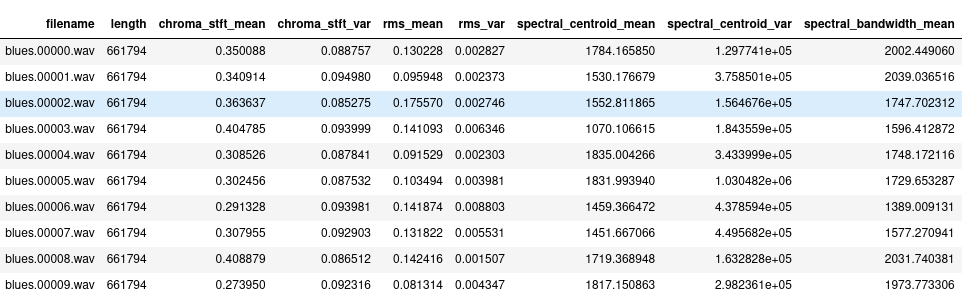
\includegraphics[width=1\textwidth]{imagenes/dataset.png}
    \end{center}
\end{frame}

\defverbatim[colored]\lstI{
\begin{lstlisting}[language=Python]
    # Seleccionamos las primeras 59 columnas.
    X = df.drop(['filename', 'label'], axis=1) 
    y = df['label'] # Seleccionamos la columna 60.
\end{lstlisting}
}

\begin{frame}{Preprocesamiento de datos}
    Dividimos nuestro conjunto en dos: 
    \begin{itemize}
        \item $X$ para los atributos característica.

        \item $y$ para las etiquetas (géneros).
    \end{itemize}
    \lstI
\end{frame}

\begin{frame}{Preprocesamiento de Datos}
    Normalizamos nuestro conjunto $X$ usando \texttt{StandardScaler}. Ésta 
    clase estándariza los datos eliminando la media y escalando los datos 
    de forma que su varianza sea igual a 1.
    \begin{center}
        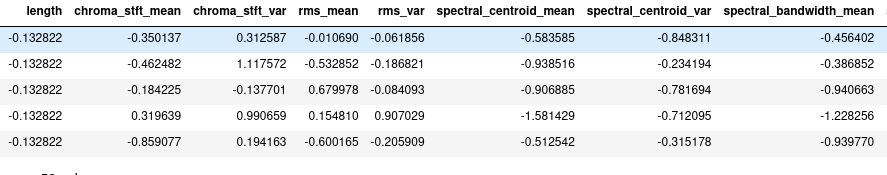
\includegraphics[width=1\textwidth]{imagenes/X.png}
    \end{center}
\end{frame}

\begin{frame}{Preprocesamiento de Datos}
    La variable de salida es un valor de string. Debemos convertirlos en 
    valores enteros entre $0$ y $9$. Esto lo podemos lograr usando la 
    clase \texttt{LabelEncoder}, pues ésta modelará la codificación 
    requerida y creará una nueva variable de salida.

    Así, obtenemos que:
    \begin{itemize}
        \item 0 $\rightarrow$ blues \quad \quad \;
        1 $\rightarrow$ classical
        \item 2 $\rightarrow$ country \quad \;
        3 $\rightarrow$ disco
        \item 4 $\rightarrow$ hiphop \quad \quad
        5 $\rightarrow$ jazz
        \item 6 $\rightarrow$ metal \quad \quad \;
        7 $\rightarrow$ pop
        \item 8 $\rightarrow$ reggae \quad \quad
        9 $\rightarrow$ rock
    \end{itemize}
\end{frame}

\begin{frame}{Preprocesamiento de Datos}
    Dividimos nuestros nuevos conjuntos de datos con un split del $80-20$ para 
    entrenamiento y prueba, respectivamente.
    \begin{center}
        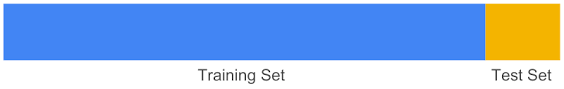
\includegraphics[width=1\textwidth]{imagenes/train-test.png}
    \end{center}
\end{frame}

\defverbatim[colored]\lstI{
\begin{lstlisting}[language=Python]
    svclassifier = SVC(kernel='linear')
    svclassifier.fit(X_train, y_train)
    y_pred = svclassifier.predict(X_test)
\end{lstlisting}
}

\begin{frame}{SVC}
\justifying
Creamos nuestro modelo SVC (usando un kernel \texttt{lineal}) y lo entrenamos.
Luego, ya podemos comenzar a realizar nuestras predicciones.
\lstI
\begin{center}
    
\includegraphics[width=0.3\textwidth]{imagenes/entrenamiento.jpg}
\end{center}
\end{frame}

\begin{frame}{SVC}
\justifying
En el conjunto de entrenamiento obtenemos un $98\%$ de precisión, mientras que 
en el conjunto de prueba obtenemos un $76\%$ de precisión.
\begin{center}
    
\includegraphics[width=0.3\textwidth]{imagenes/feliz.png}
\end{center}
\end{frame}

\begin{frame}{PCA}
    \justifying
    Usaremos PCA para obtener la lista de atributos que tienen mayor varianza 
    (mayor poder explicativo). Éstos serán las componentes principales.
    \begin{figure}
        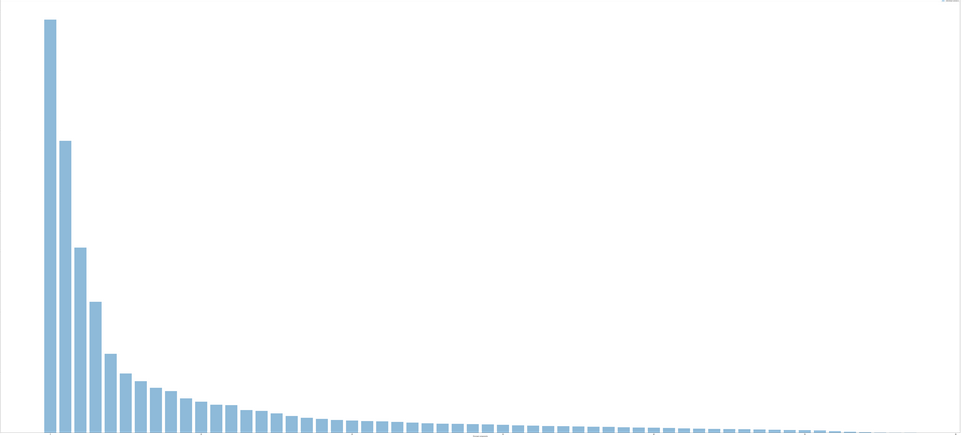
\includegraphics[width=1\textwidth]{imagenes/components1.png}
        \caption{Variance ratio vs Principal components}
    \end{figure}
\end{frame}
		
\begin{frame}{PCA}
\justifying
\begin{figure}
    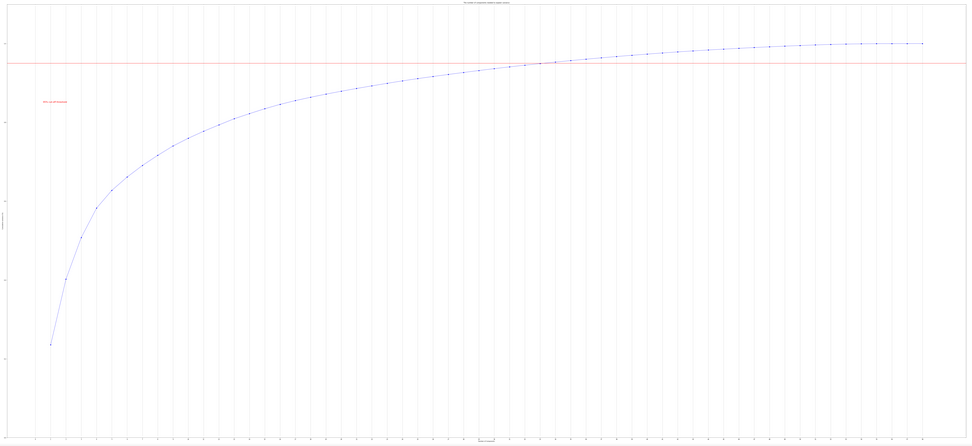
\includegraphics[width=1\textwidth]{imagenes/components2.png}
    \caption{Cumulative variance vs The number of components needed to explain variance}
\end{figure}
\end{frame}

\begin{frame}{PCA}
\justifying
Obtenemos que el número de componentes para obtener una varianza explicada 
del $98\%$ es de $43$.
\begin{center}
    
\includegraphics[width=0.25\textwidth]{imagenes/componentes3.jpg}
\end{center}
\end{frame}

\defverbatim[colored]\lstI{
\begin{lstlisting}[language=Python]
    svclassifier = SVC(kernel='linear')
    svclassifier.fit(X_train, y_train)
    y_pred = svclassifier.predict(X_test)
\end{lstlisting}
}

\begin{frame}{PCA}
    \justifying
    Instanciamos un objeto de PCA y lo aplicamos.
    \lstI
    Finalmente, usamos SVC con este nuevo conjunto reducido.
\end{frame}

\begin{frame}{PCA}
    \justifying
    En el conjunto de entrenamiento obtenemos un $96\%$ de precisión, mientras que 
    en el conjunto de prueba obtenemos un $74\%$ de precisión.
    \begin{center}
        
\includegraphics[width=0.3\textwidth]{imagenes/feliz.png}
    \end{center}
    \end{frame}
	
\section{Resultados}
\begin{frame}{Resultados}
    \justifying
    Obtenemos que gracias a PCA logramos una precisión muy buena con $43$
    componentes principales. 
    \begin{itemize}
        \item SVC 
        \begin{equation*}
            98\% \; \; \texttt{train} \quad \quad 76\% \; \; \texttt{test}
        \end{equation*}

        \item PCA/SVC
        \begin{equation*}
            96\% \; \; \texttt{train} \quad \quad 74\% \; \; \texttt{test}
        \end{equation*}
    \end{itemize}
\end{frame}

\begin{frame}{Resultados}
    \begin{figure}
    \centering
    \subfloat[SVC]
    {{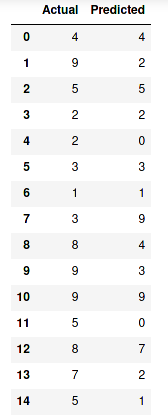
\includegraphics[width=2.4cm]{imagenes/svc-resultados.png}}}%
    \qquad
    \subfloat[PCA]
    {{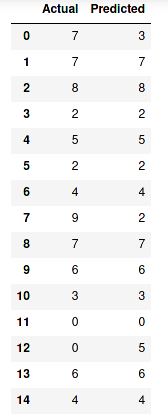
\includegraphics[width=2.4cm]{imagenes/pca-resultados.png}}}%
    \caption{Predicciones}%
    \label{fig:example}%
    \end{figure}
\end{frame}

\begin{frame}{Resultados}
    \begin{figure}
    \centering
    \subfloat[SVC]
    {{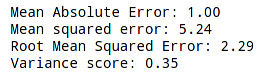
\includegraphics[width=5cm]{imagenes/svc-valores.png}}}%
    \qquad
    \subfloat[PCA]
    {{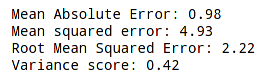
\includegraphics[width=5cm]{imagenes/pca-valores.png}}}%
    \caption{Precisión}%
    \label{fig:example}%
    \end{figure}
\end{frame}

\section{Conclusiones}
\begin{frame}{Conclusiones}
\centering
    
\includegraphics[width=0.5\textwidth]{imagenes/homero.jpg}
\end{frame}
	
\end{document}
